\section{Results}


\subsection{Depletion calculation time}

For 100 sets of
burnup and enrichment depletion calculations,
the model takes 0.12 seconds, while
searching the database for an assembly
with the closest burnup and enrichment (using Pandas read csv)
takes 21.8 seconds.

\subsection{U.S. \gls{UNF} inventory comparison}


The Unified database contains discharged assembly data
from nuclear reactors in the United States up to May of
2013. 


\begin{table}[h]
    \centering
    \begin{tabular}{lrrr}
        \hline
        Metric & Data & Recipe & Prediction \\
        \hline
        $^{239}Pu$ mass [t] & 321.02 & 315.40 & 319.28\\
        $^{137}Cs$ mass [t] & 40.72 & 38.85 & 40.29 \\
        $^{235}U$ mass [t] & 478.74 & 468.11 & 457.10\\
        $^{238}U$ mass [t] & 42,379 & 42,399 & 42,422\\
        Decay Heat [MW] & 193.59 & 177.28 & 192.00 \\
        Activity [Bq] & $2.80e21$ & $2.52e21$ & $2.74e21$ \\
        \hline
    \end{tabular}
    \caption{Comparison of \gls{PWR} \gls{UNF} inventory in the U.S.,
             using the Unified database.}
\end{table}


\begin{table}[h]
    \centering
    \begin{tabular}{lcrrr}
        \hline
        Metric & Year & HR case & Prediction case  & Error [\%] \\
        \hline
        \multirow{3}{*}{\shortstack{Decay \\ Heat}} & 2020 & 41.01 & 40.83 & ???? \\
                                                    & 2100 & ???? & ???? & ???? \\
                                                    & 3100 & ???? & ???? & ???? \\
        \hline
        \multirow{3}{*}{\shortstack{Activity}} & 2020 & 4.67e20 & 4.62e20 & ???? \\
                                               & 2100 & ???? & ???? & ???? \\
                                               & 3100 & ???? & ???? & ???? \\
        \hline
    \end{tabular}
    \caption{Decay heat and radioactivity values and errors for years 2020, 2100, and 3100.}
    \label{tab:wm}
\end{table}

\begin{figure}
    \centering
    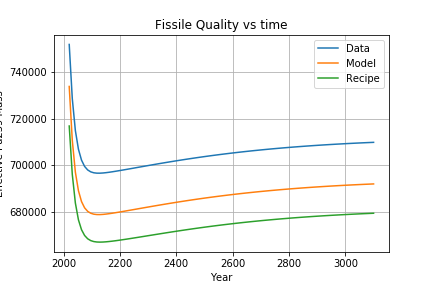
\includegraphics[width=\textwidth]{fiss.png}
    \caption{Effective Pu-239 mass value of \gls{UNF} inventory generated by
             Unifed database, average recipe, and the prediction model. }
    \label{fig:fiss}
\end{figure}

\begin{figure}
    \centering
    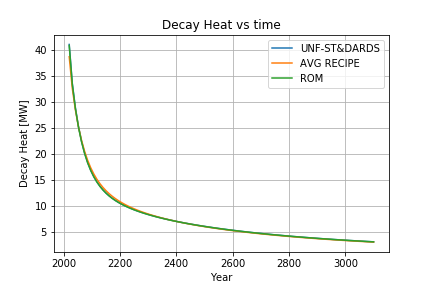
\includegraphics[width=\textwidth]{heat.png}
    \caption{Decay heat of \gls{UNF} inventory generated by
             Unifed database, average recipe, and the prediction model. }
    \label{fig:heat}
\end{figure}

\begin{figure}
    \centering
    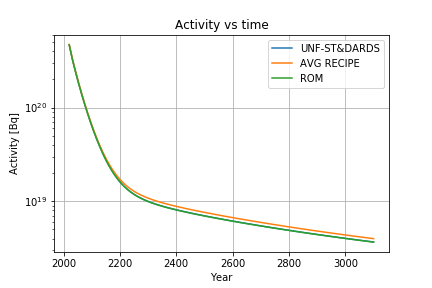
\includegraphics[width=\textwidth]{activity.png}
    \caption{Activity of \gls{UNF} inventory generated by
             Unifed database, average recipe, and the prediction model. }
    \label{fig:activity}
\end{figure}

\begin{figure}
    \centering
    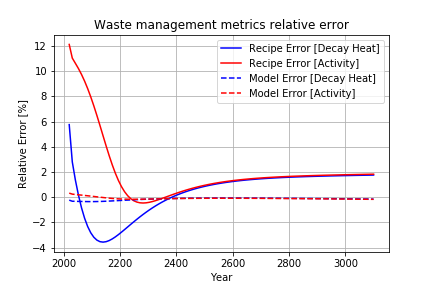
\includegraphics[width=\textwidth]{ha_err.png}
    \caption{Relative error of waste management metrics for \gls{UNF} inventory
             generated by the average recipe, and the prediction model.}
    \label{fig:ha_err}
\end{figure}